% =====================================================================
%  Biên dịch:  xelatex BAO_CAO.tex && xelatex BAO_CAO.tex
%  (chạy hai lần để Mục lục và tham chiếu chéo cập nhật đúng)
%
%  BẮT BUỘC dùng XeLaTeX hoặc LuaLaTeX, không dùng pdfLaTeX,
%  vì tài liệu nạp font Unicode có dấu tiếng Việt qua fontspec.
%
%  Trên Overleaf: Menu -> Compiler -> XeLaTeX
% =====================================================================
\documentclass[11pt,a4paper]{article}

\usepackage{fontspec}
% Tự dò font: ưu tiên TeX Gyre Termes (bản Times của TeX Live, có trên Overleaf),
% nếu máy không có thì lùi về Liberation Serif rồi DejaVu Serif.
\IfFontExistsTF{TeX Gyre Termes}{\setmainfont{TeX Gyre Termes}}{%
  \IfFontExistsTF{Liberation Serif}{\setmainfont{Liberation Serif}}{%
    \setmainfont{DejaVu Serif}}}
\IfFontExistsTF{TeX Gyre Heros}{\setsansfont{TeX Gyre Heros}}{%
  \IfFontExistsTF{Liberation Sans}{\setsansfont{Liberation Sans}}{%
    \setsansfont{DejaVu Sans}}}
\IfFontExistsTF{TeX Gyre Cursor}{\setmonofont{TeX Gyre Cursor}[Scale=0.88]}{%
  \IfFontExistsTF{Liberation Mono}{\setmonofont{Liberation Mono}[Scale=0.88]}{%
    \setmonofont{DejaVu Sans Mono}[Scale=0.84]}}

\usepackage[a4paper,margin=2.3cm]{geometry}
\usepackage{amsmath,amssymb}
\usepackage{booktabs}
\usepackage{tabularx}
\usepackage{multirow}
\usepackage{graphicx}
\usepackage{caption}
\usepackage{float}
\usepackage{xcolor}
\usepackage{enumitem}
\usepackage{titlesec}
\usepackage{abstract}

% Trích dẫn [n] và URL hiển thị màu xanh; tham chiếu nội bộ (Bảng, Hình, Mục)
% giữ màu đen để không làm rối trang.
\definecolor{citeblue}{RGB}{0,84,180}
\usepackage[unicode,colorlinks=true,
            citecolor=citeblue,
            urlcolor=citeblue,
            linkcolor=black,
            filecolor=citeblue]{hyperref}

% ---- Nhãn tiếng Việt ----
\renewcommand{\abstractname}{TÓM TẮT}
\renewcommand{\refname}{TÀI LIỆU THAM KHẢO}
\renewcommand{\contentsname}{MỤC LỤC}
\renewcommand{\figurename}{Hình}
\renewcommand{\tablename}{Bảng}
\renewcommand{\appendixname}{Phụ lục}

% ---- Định dạng đề mục ----
\titleformat{\section}
  {\normalfont\large\bfseries\MakeUppercase}{\thesection.}{0.7em}{}
\titleformat{\subsection}
  {\normalfont\normalsize\bfseries}{\thesubsection.}{0.6em}{}
\titleformat{\subsubsection}
  {\normalfont\normalsize\itshape}{\thesubsubsection.}{0.6em}{}
\titlespacing*{\section}{0pt}{1.6em}{0.8em}
\titlespacing*{\subsection}{0pt}{1.2em}{0.5em}

\setlength{\parskip}{0.45em}
\setlength{\parindent}{0pt}
\captionsetup{font=small,labelfont=bf,skip=6pt}
\captionsetup[table]{position=top}

% ---- Lệnh tắt ----
\newcommand{\file}[1]{\texttt{\small #1}}
\newcommand{\ours}{\textbf{Ours}}
\newcommand{\best}[1]{\textbf{#1}}
\renewcommand{\arraystretch}{1.15}

% =====================================================================
\begin{document}

\begin{center}
{\LARGE\bfseries So sánh kiến trúc Transformer và Seq2Seq--Attention\\[0.3em]
cho dịch máy Anh--Việt trên ngữ liệu IWSLT'15}

\vspace{1.3em}
{\large\bfseries Lê Hoàng Quân}\\[0.4em]
Mã sinh viên: 24022433\\[0.4em]
\href{https://github.com/quanai06/machine_translate}%
{\file{github.com/quanai06/machine\_translate}}
\end{center}

\vspace{1.2em}

\begin{abstract}
\noindent\small
Báo cáo cài đặt lại hai kiến trúc Neural Machine Translation (NMT) và so sánh
chúng trên cùng ngữ liệu song ngữ Anh--Việt IWSLT'15. Trường hợp thứ nhất là
Transformer~\cite{vaswani2017}, kiến trúc Encoder--Decoder hoàn toàn dựa trên
Self-Attention. Trường hợp thứ hai là Seq2Seq dùng Long Short-Term Memory (LSTM)
kèm Global Attention~\cite{luong2015emnlp}, tức kiến trúc nền tảng của bộ mã
nguồn tham chiếu TF-NMT~\cite{tfnmt}. Cả hai được cài đặt bằng PyTorch và dùng
chung Tokenizer, chung cách chia Batch, chung công thức tính BLEU, nhằm bảo đảm
chênh lệch quan sát được phản ánh kiến trúc chứ không phản ánh kỹ thuật huấn
luyện. Trên tập kiểm thử tst2013, mô hình Transformer đạt 30,35 BLEU với Beam
Search, mô hình Seq2Seq đạt 27,81 BLEU. Cả hai đều vượt các mốc đã công bố trên
cùng ngữ liệu, trong đó bản Seq2Seq vượt chính hệ thống mà nó tái hiện 1,71 điểm
BLEU. Báo cáo cũng chỉ ra rằng lợi thế tốc độ huấn luyện thường được gán cho
Transformer không xuất hiện ở quy mô mô hình và phần cứng của thí nghiệm này.

\vspace{0.7em}
\noindent\textbf{Từ khoá:} Neural Machine Translation, Transformer,
Sequence-to-Sequence, Attention, Byte Pair Encoding, BLEU, IWSLT'15,
Anh--Việt, Low-Resource.
\end{abstract}

\vspace{0.6em}
\hrule
\vspace{0.4em}

{\small\tableofcontents}

\vspace{0.4em}
\hrule

% =====================================================================
\section{Mô tả hai trường hợp nghiên cứu}
\label{sec:mota}

\subsection{Bài toán và ngữ liệu}

Bài toán là dịch tự động từ tiếng Anh sang tiếng Việt ở miền phụ đề hội thoại
TED Talks. Ngữ liệu là IWSLT'15 English--Vietnamese, được phát hành kèm hệ thống
Stanford-NMT~\cite{luong2015iwslt}. Đây là ngữ liệu chuẩn cho cặp ngôn ngữ này
và được hầu hết các nghiên cứu sau đó dùng làm mốc đối chiếu.

\begin{table}[H]
\centering
\caption{Phân chia ngữ liệu IWSLT'15 English--Vietnamese}
\label{tab:data}
\begin{tabular}{llrr}
\toprule
\textbf{Tập} & \textbf{Tệp} & \textbf{Số câu} & \textbf{Vai trò} \\
\midrule
Huấn luyện & \file{train.\{en,vi\}}   & 133.317 & Training \\
Phát triển & \file{tst2012.\{en,vi\}} & 1.553   & Validation, chọn Checkpoint \\
Kiểm thử   & \file{tst2013.\{en,vi\}} & 1.268   & Test, báo cáo BLEU \\
\bottomrule
\end{tabular}
\end{table}

Sau khi loại các câu dài quá 100 đơn vị Subword, tập huấn luyện thực tế còn
132.010 câu. Ngữ liệu được phát hành ở dạng đã tách từ theo quy ước Moses, và
toàn bộ điểm BLEU trong tài liệu tham khảo đều báo cáo trên tst2013. Báo cáo giữ
nguyên quy ước này để bảo đảm khả năng đối chiếu.

\begin{table}[H]
\centering
\caption{Thống kê ngữ liệu huấn luyện}
\label{tab:stats}
\begin{tabular}{lrrrrr}
\toprule
\textbf{Phía} & \textbf{Câu} & \textbf{Token} & \textbf{Vocab thô}
& \textbf{Độ dài TB} & \textbf{Hapax} \\
\midrule
Tiếng Anh  & 133.317 & 2.706.255 & 54.169 & 20,3 & 21.912 \small(40\%) \\
Tiếng Việt & 133.317 & 3.311.508 & 25.615 & 24,8 & 11.298 \small(44\%) \\
\bottomrule
\end{tabular}
\end{table}

Bảng~\ref{tab:stats} cho thấy hai đặc điểm chi phối các quyết định thiết kế ở
Mục~\ref{sec:phuongphap}. Thứ nhất, 40\% từ vựng phía tiếng Anh chỉ xuất hiện
đúng một lần (Hapax Legomenon). Với từ điển cố định ở mức từ, phần lớn số này sẽ
trở thành ký hiệu \file{<unk>}; đây chính là Rare Word Problem mà BPE~\cite{sennrich2016}
được đề xuất để giải quyết. Thứ hai, câu tiếng Việt dài hơn câu tiếng Anh khoảng
22\% tính theo đơn vị phân tách bằng khoảng trắng, do tiếng Việt viết rời từng
âm tiết.

\subsection{Trường hợp 1: Transformer}

Transformer~\cite{vaswani2017} là kiến trúc Encoder--Decoder hoàn toàn dựa trên
Self-Attention, không dùng thành phần hồi tiếp. Điểm mấu chốt nằm ở độ dài đường
đi của tín hiệu: trong mạng hồi tiếp, thông tin giữa hai vị trí $i$ và $j$ phải
truyền qua $|i-j|$ bước, trong khi Self-Attention chỉ cần một bước. Hệ quả là
Gradient không suy giảm theo khoảng cách, đồng thời toàn bộ chuỗi đích có thể
huấn luyện song song thay vì tuần tự.

Nguồn tham chiếu ban đầu là notebook \file{demo\_transformer.ipynb}.

\subsection{Trường hợp 2: Seq2Seq kèm Attention}

Trường hợp thứ hai là mạng Encoder--Decoder dùng LSTM kèm Global
Attention~\cite{luong2015emnlp}, kiến trúc đứng sau bộ mã nguồn
TF-NMT~\cite{tfnmt} vốn công bố mốc 26,1 BLEU cho cặp Anh--Việt trên tst2013.

Kiến trúc này là kết quả của một chuỗi cải tiến. Seq2Seq~\cite{sutskever2014}
đề xuất khung Encoder--Decoder trong đó câu nguồn được nén vào một vector kích
thước cố định, nhưng chất lượng suy giảm mạnh theo độ dài câu vì một vector
không đủ chứa thông tin của câu dài. RNNSearch~\cite{bahdanau2015} gỡ nút thắt
này bằng cách cho Decoder truy cập lại toàn bộ trạng thái Encoder thông qua
trọng số Attention học được. Global Attention~\cite{luong2015emnlp} sau đó đơn
giản hoá hàm tính điểm và bổ sung cơ chế Input Feeding.

Cần lưu ý rằng TF-NMT~\cite{tfnmt} được viết bằng TensorFlow 1.x và phụ thuộc
vào mô-đun \file{tf.contrib.seq2seq}. Mô-đun \file{tf.contrib} đã bị loại bỏ
khỏi TensorFlow 2.0, còn TensorFlow Addons, nơi các API này chuyển sang, đã kết
thúc vòng đời vào tháng 5 năm 2024. Do đó mã nguồn gốc không còn chạy được trên
môi trường hiện tại, và việc cài đặt lại là bắt buộc chứ không phải lựa chọn.

\subsection{Lựa chọn Framework}

Cả hai trường hợp đều cài đặt bằng PyTorch, vì ba lý do. Thứ nhất, như đã nêu,
mã nguồn tham chiếu của trường hợp 2 không còn chạy được nên dù chọn TensorFlow
thì vẫn phải viết lại từ đầu. Thứ hai, nếu hai trường hợp dùng hai Framework
khác nhau thì mọi chênh lệch về thời gian huấn luyện và bộ nhớ sẽ lẫn giữa yếu
tố kiến trúc và yếu tố Framework, khiến phép so sánh mất giá trị. Thứ ba, vòng
huấn luyện tường minh của PyTorch cho phép đo chính xác thời gian mỗi Epoch,
Throughput và bộ nhớ đỉnh, vốn là một phần yêu cầu của bài toán.

% =====================================================================
\section{Phương pháp}
\label{sec:phuongphap}

\subsection{Các thành phần dùng chung}

Điều kiện tiên quyết để phép so sánh có giá trị là hai mô hình được đối xử như
nhau ở mọi khâu ngoài kiến trúc. Bảng~\ref{tab:shared} liệt kê các thành phần
dùng chung và căn cứ tương ứng.

\begin{table}[H]
\centering
\small
\caption{Các thành phần dùng chung cho cả hai trường hợp}
\label{tab:shared}
\begin{tabularx}{\textwidth}{lXc}
\toprule
\textbf{Thành phần} & \textbf{Cấu hình} & \textbf{Căn cứ} \\
\midrule
Tokenizer & SentencePiece BPE, 8.000 đơn vị mỗi phía & \cite{sennrich2016} \\
Tách từ tiếng Việt & Không dùng & \cite{phanvu2017,phanvu2019} \\
Chia Batch & Theo số Token, tối đa 8.192 Token đích & \cite{ott2018} \\
Hàm mất mát & Cross-Entropy, Label Smoothing $\varepsilon = 0{,}1$ & \cite{vaswani2017} \\
Mixed Precision & fp16 qua \file{torch.amp} & \cite{ott2018} \\
Length Penalty & $((5+|Y|)/6)^{\alpha}$, $\alpha = 1{,}0$ & \cite{wu2016} \\
Chọn Checkpoint & Theo BLEU trên tst2012, Early Stopping sau 5 Epoch & --- \\
\bottomrule
\end{tabularx}
\end{table}

Ba lựa chọn cần giải thích thêm.

\textbf{Kích thước Vocab.} Mức 8.000 Subword mỗi phía được chọn theo quy mô dữ
liệu chứ không theo mặc định thông dụng. Với 133 nghìn câu, mức 32.000 Subword
là quá lớn vì các Subword hiếm sẽ chỉ xuất hiện vài lần trong toàn bộ quá trình
huấn luyện.

\textbf{Bỏ bước tách từ tiếng Việt.} Kết quả thực nghiệm trên chính cặp
Anh--Việt~\cite{phanvu2017} cho thấy bước tách từ (Word Segmentation) là không
cần thiết đối với NMT dùng Subword, dù nó có ích rõ rệt với Statistical Machine
Translation (SMT). Kết luận này được kiểm chứng lại trong nghiên cứu mở
rộng~\cite{phanvu2019}.

\textbf{Cách tính BLEU.} Ngữ liệu phát hành ở dạng đã tách từ theo Moses, và mọi
con số công bố trên ngữ liệu này là Tokenized BLEU tính bằng \file{multi-bleu.perl}.
Công cụ \file{sacrebleu} mặc định tokenize lại bằng \file{13a}, nên đưa thẳng
văn bản đã tách từ vào sẽ cho một con số thứ ba không so được với gì. Báo cáo
dùng \file{sacrebleu} với tham số \file{tokenize="none"}, tương đương
\file{multi-bleu.perl}, và bổ sung thêm Detokenized BLEU cùng chrF2.

\subsection{Trường hợp 1: Transformer}

\begin{table}[H]
\centering
\small
\caption{Siêu tham số của mô hình Transformer}
\label{tab:cfg-tf}
\begin{tabular}{llc}
\toprule
\textbf{Tham số} & \textbf{Giá trị} & \textbf{Căn cứ} \\
\midrule
$d_{\text{model}}$ / số Head       & 512 / 4                    & \cite{vaswani2017} \\
Số lớp                             & 6 Encoder + 6 Decoder      & \cite{vaswani2017} \\
$d_{\text{ff}}$                    & 1024                       & giảm nửa so với Base \\
Dropout                            & 0,3                        & cao hơn mức 0,1 của Base \\
Chuẩn hoá                          & Pre-Norm                   & \cite{nguyen2019} \\
Positional Encoding                & Sin/Cos, không học         & \cite{vaswani2017} \\
Weight Tying                       & Có                         & --- \\
Learning Rate Schedule             & Inverse-Sqrt, 4.000 Warmup & \cite{vaswani2017} \\
Optimizer                          & AdamW, $\beta=(0{,}9;\,0{,}98)$ & \cite{vaswani2017} \\
\midrule
\textbf{Tổng tham số}              & \textbf{39.737.344}        & \\
\bottomrule
\end{tabular}
\end{table}

Hai điều chỉnh so với cấu hình gốc cần được giải thích.

\textbf{Không dùng cấu hình Base.} Cấu hình Base~\cite{vaswani2017} có
$d_{\text{ff}} = 2048$, Dropout 0,1 và khoảng 65 triệu tham số, được huấn luyện
trên WMT'14 English--German với 4,5 triệu câu. IWSLT'15 chỉ có 133 nghìn câu, ít
hơn 34 lần. Sao chép nguyên cấu hình từ bối cảnh dữ liệu lớn sang bối cảnh
Low-Resource dẫn tới Overfitting. Cấu hình dùng ở đây thu hẹp mạng Feed-Forward
xuống một nửa và nâng Dropout lên 0,3.

\textbf{Dùng Pre-Norm thay vì Post-Norm.} Đặt Layer Normalization trước mỗi
Sublayer giúp huấn luyện hội tụ ổn định ở Learning Rate lớn mà không cần giai
đoạn Warmup dài~\cite{nguyen2019}. Điểm đáng chú ý là ở bối cảnh dữ liệu lớn
(WMT'14 English--German), Pre-Norm lại làm \emph{giảm} chất lượng. Nghĩa là đây
là một đánh đổi phụ thuộc lượng dữ liệu chứ không phải cải tiến phổ quát. Kết
quả TwT~\cite{nguyen2019} được đo trực tiếp trên chính ngữ liệu IWSLT'15
English--Vietnamese và lập mốc 32,8 BLEU, cao nhất được công bố ở thời điểm đó.

\subsection{Trường hợp 2: Seq2Seq kèm Attention}

Cấu hình bám theo mốc chuẩn công bố trong TF-NMT~\cite{tfnmt}.

\begin{table}[H]
\centering
\small
\caption{Siêu tham số của mô hình Seq2Seq kèm Attention}
\label{tab:cfg-s2s}
\begin{tabular}{llc}
\toprule
\textbf{Tham số} & \textbf{Giá trị} & \textbf{Căn cứ} \\
\midrule
Encoder        & 1 lớp Bi-LSTM, 512 đơn vị          & \cite{tfnmt} \\
Decoder        & 2 lớp LSTM, 512 đơn vị             & \cite{tfnmt} \\
Attention      & Global Attention, hàm điểm \file{general}, có Scale & \cite{luong2015emnlp,tfnmt} \\
Input Feeding  & Có                                 & \cite{luong2015emnlp} \\
Dropout        & 0,2                                & \cite{tfnmt} \\
Gradient Clipping & 5,0                             & \cite{tfnmt} \\
Beam Size      & 10                                 & \cite{tfnmt} \\
Optimizer      & Adam, Learning Rate $10^{-3}$      & xem ghi chú \\
\midrule
\textbf{Tổng tham số} & \textbf{20.005.889}          & \\
\bottomrule
\end{tabular}
\end{table}

Ba thành phần được lấy trực tiếp từ Global Attention~\cite{luong2015emnlp}.

\textbf{Hàm tính điểm \file{general}.} Điểm Attention giữa trạng thái Decoder
$h_t$ và trạng thái Encoder $h_s$ được tính theo
\[
\text{score}(h_t, h_s) = h_t^{\top} W_a\, h_s .
\]
Ba biến thể \file{dot}, \file{general} và \file{concat} được khảo sát
trong~\cite{luong2015emnlp}; biến thể \file{general} cho kết quả tốt nhất và
cũng là mặc định của TF-NMT~\cite{tfnmt}. Bản cài đặt trong báo cáo có đủ cả ba,
mặc định dùng \file{general}.

\textbf{Input Feeding.} Vector Attentional $\tilde{h}_t$ được nối vào đầu vào
của bước sinh kế tiếp, giúp Decoder ghi nhớ vị trí đã căn chỉnh ở bước trước,
qua đó tránh dịch lặp hoặc bỏ sót. Đây là điểm khác biệt so với
RNNSearch~\cite{bahdanau2015}, và cũng là nguyên nhân buộc Decoder chạy tuần tự
theo từng bước thời gian.

\textbf{Length Penalty.} Log-Probability luôn giảm theo độ dài chuỗi nên Beam
Search thuần thiên vị câu ngắn, kéo Brevity Penalty của BLEU xuống. Công thức
chuẩn hoá $((5+|Y|)/6)^{\alpha}$ của GNMT~\cite{wu2016} được áp dụng cho cả hai
trường hợp.

\textbf{Ghi chú về Optimizer.} TF-NMT~\cite{tfnmt} dùng Stochastic Gradient
Descent (SGD) với Learning Rate 1,0. Báo cáo dùng Adam làm mặc định vì trường
hợp 1 cũng dùng Adam; nếu hai mô hình chạy hai họ thuật toán tối ưu khác nhau
thì chênh lệch quan sát được sẽ lẫn giữa yếu tố kiến trúc và yếu tố tối ưu hoá.
Mã nguồn vẫn cho phép tái hiện đúng cấu hình gốc bằng tham số
\file{--optimizer sgd --lr 1.0}.

\subsection{Quy trình kiểm chứng cài đặt}

Trước khi huấn luyện đầy đủ, hai kiểm tra được thực hiện và cả hai đều phát hiện
lỗi thật.

\textbf{Kiểm tra Mixed Precision.} Lỗi lệch kiểu dữ liệu giữa fp16 và fp32 không
biểu hiện khi chạy trên CPU không bật Mixed Precision, nhưng làm hỏng ngay lần
huấn luyện đầu tiên trên GPU. Kiểm tra này phát hiện rằng các phép chiếu khởi
tạo trạng thái Decoder của trường hợp 2 chạy dưới Autocast nên sinh ra trạng
thái fp16, trong khi đầu vào LSTM bị ép về fp32, mà \file{nn.LSTM} yêu cầu hai
thứ này cùng kiểu.

\textbf{Kiểm tra Overfitting có chủ đích.} Mô hình được yêu cầu học thuộc 120
câu rồi chấm BLEU trên chính 120 câu đó; một cài đặt đúng phải đạt trên 80 BLEU.
Kiểm tra này phát hiện lỗi thứ hai: bản cài đặt đầu tiên chuyển nguyên tham số
\file{init\_weight = 0.1} của TF-NMT~\cite{tfnmt} sang PyTorch, khiến Logit lúc
khởi tạo có độ lệch chuẩn chỉ khoảng 0,005. Hàm Softmax khi đó gần như phân bố
đều tuyệt đối trên 8.000 lớp, vùng Gradient rất phẳng, và mô hình chậm hơn
Transformer khoảng 10 lần chỉ để thoát khỏi vùng này. Sau khi khởi tạo lại theo
Fan-In của từng lớp, Perplexity sau 200 bước giảm từ 7,8 xuống 2,08. Lỗi này
không gây dừng chương trình mà chỉ làm hội tụ chậm, nên một lần huấn luyện dài
sẽ che mất nó.

% =====================================================================
\section{Thực nghiệm và kết quả}
\label{sec:ketqua}

\subsection{Cấu hình thí nghiệm}

Toàn bộ thí nghiệm chạy trên Google Colab với GPU NVIDIA Tesla T4 (16~GB). Hai
mô hình dùng chung Tokenizer, chung cách chia Batch, chung công thức BLEU và
cùng tập kiểm thử tst2013.

\subsection{So sánh với các hệ thống trên cùng ngữ liệu}

Bảng~\ref{tab:sota} đối chiếu hai mô hình của báo cáo với các công trình khác
trên cặp ngôn ngữ Anh--Việt, tất cả đều đánh giá chiều English$\rightarrow$Vietnamese
trên tập tst2013 của IWSLT'15. Các hệ thống được nhóm theo họ kiến trúc: SMT,
NMT dựa trên mạng hồi tiếp, và NMT dựa trên Transformer.

\begin{table}[H]
\centering
\footnotesize
\setlength{\tabcolsep}{4.5pt}
\caption{Đối chiếu các công trình dịch máy Anh--Việt, chiều
English$\rightarrow$Vietnamese, tập kiểm thử tst2013 (IWSLT'15). Cột \emph{Dữ
liệu} là số câu song ngữ dùng để huấn luyện. Số in đậm là kết quả tốt nhất trong
mỗi họ kiến trúc; \ours{} là hai mô hình của báo cáo này. $^\dagger$~dùng tập
kiểm thử tst2015 thay vì tst2013. $^\ddagger$~huấn luyện trên ngữ liệu riêng lớn
hơn nhiều và tính điểm bằng sacreBLEU không phân biệt hoa thường, nên không so
trực tiếp được với các dòng còn lại.}
\label{tab:sota}
\begin{tabular}{llllrrr}
\toprule
\multirow{2}{*}{\textbf{Hệ thống}} & \multirow{2}{*}{\textbf{Kiến trúc}}
& \multirow{2}{*}{\textbf{Đơn vị}} & \multirow{2}{*}{\textbf{Dữ liệu}}
& \textbf{dev} & \multicolumn{2}{c}{\textbf{test (tst2013)}} \\
\cmidrule(lr){5-5}\cmidrule(lr){6-7}
 & & & & tst2012 & Greedy & Beam \\
\midrule
\multicolumn{7}{l}{\textit{Statistical Machine Translation}} \\
PBSMT~\cite{tran2015}
  & Phrase-Based + LM 4-gram & Từ (VnTokenizer) & 122k & --- & --- & 23,15$^\dagger$ \\
\midrule
\multicolumn{7}{l}{\textit{NMT dựa trên mạng hồi tiếp}} \\
Stanford-NMT~\cite{luong2015iwslt}
  & RNN + Attention & Từ & 133k & --- & --- & 23,3 \\
TF-NMT~\cite{tfnmt}
  & LSTM + Global Attn & Từ (17k/7,7k) & 133k & 23,8 & 25,5 & 26,1 \\
SAWR-Base~\cite{zhang2019}
  & Seq2Seq baseline & BPE & 133k & --- & --- & 28,29 \\
SAWR~\cite{zhang2019}
  & Seq2Seq + Syntax-Aware & BPE & 133k & --- & --- & \best{29,09} \\
\ours{}-S2S
  & LSTM + Global Attn & BPE 8k & 132k & 23,96 & 26,64 & 27,81 \\
\midrule
\multicolumn{7}{l}{\textit{NMT dựa trên Transformer}} \\
\ours{}-TF
  & Transformer + Pre-Norm & BPE 8k & 132k & 26,42 & 29,47 & 30,35 \\
TwT~\cite{nguyen2019}
  & Transformer + ScaleNorm & BPE & 133k & --- & --- & \best{32,8} \\
\midrule
\multicolumn{7}{l}{\textit{Huấn luyện trên ngữ liệu lớn hơn, chỉ để tham khảo}} \\
Phan-Vu~\cite{phanvu2019}
  & Bi-LSTM 1024, 98M tham số & BPE 32k & 886k & 34,77 & --- & 37,00$^\ddagger$ \\
\bottomrule
\end{tabular}
\end{table}

Bốn ghi chú khi đọc Bảng~\ref{tab:sota}.

\textbf{PBSMT}~\cite{tran2015} là hệ thống dự thi cùng đợt đánh giá IWSLT 2015
đã sinh ra ngữ liệu này, in ở trang 80--83 cùng kỷ yếu với
Stanford-NMT~\cite{luong2015iwslt} (trang 76--79). Đóng góp chính không nằm ở mô
hình dịch mà ở việc mở rộng dữ liệu đơn ngữ cho Language Model, cụ thể là thu
thập \textbf{1~GB} văn bản báo điện tử tiếng Việt; ba lần chạy chỉ khác nhau ở
lượng dữ liệu đơn ngữ và BLEU tăng đều từ \textbf{22,70} lên \textbf{23,15}. Con
số này đo trên tập \file{TED.tst2015} (1.046 câu) chứ không phải tst2013, nên
chỉ mang tính tham chiếu.

\textbf{SAWR}~\cite{zhang2019} tích hợp biểu diễn từ nhận biết cú pháp
(Syntax-Aware Word Representations) vào Encoder, nâng baseline từ \textbf{28,29}
lên \textbf{29,09} BLEU, tức \textbf{+0,80} điểm. Đây là mốc hữu ích vì baseline
của công trình này (\textbf{28,29}) mạnh hơn TF-NMT~\cite{tfnmt} khá nhiều dù
cùng dùng 133 nghìn câu, cho thấy khoảng cách giữa các bản cài đặt Seq2Seq trên
cùng ngữ liệu là đáng kể.

\textbf{Phan-Vu}~\cite{phanvu2019} đạt \textbf{37,00} BLEU nhưng huấn luyện trên
ngữ liệu tự thu thập \textbf{886.224} câu, gấp \textbf{6,6} lần IWSLT'15, với mô
hình \textbf{98} triệu tham số. Công trình này còn tính điểm bằng sacreBLEU
không phân biệt hoa thường thay vì Tokenized BLEU. Vì cả hai lý do đó, con số
37,00 không so trực tiếp được với các dòng còn lại và chỉ đưa vào để cho thấy
trần hiệu năng khi có thêm dữ liệu.

\textbf{Vị trí của hai mô hình trong báo cáo.} \ours{}-S2S đạt \textbf{27,81},
vượt TF-NMT~\cite{tfnmt} là hệ thống mà nó tái hiện, nhưng còn kém baseline
Seq2Seq của SAWR~\cite{zhang2019}. \ours{}-TF đạt \textbf{30,35}, vượt cả
SAWR~\cite{zhang2019} và đứng thứ hai trong nhóm huấn luyện trên 133 nghìn câu,
chỉ sau TwT~\cite{nguyen2019}.

\subsection{Benchmark chi tiết hai trường hợp}

Bảng~\ref{tab:benchmark} trình bày toàn bộ số đo của hai mô hình trong cùng điều
kiện. Chỉ số nào càng cao càng tốt được đánh dấu $\uparrow$, càng thấp càng tốt
đánh dấu $\downarrow$.

\begin{table}[H]
\centering
\small
\caption{Benchmark chi tiết hai trường hợp trên cùng ngữ liệu, cùng phần cứng
Tesla T4. Số in đậm là kết quả tốt hơn.}
\label{tab:benchmark}
\begin{tabular}{ll rr}
\toprule
\textbf{Nhóm} & \textbf{Chỉ số} & \ours{}\textbf{-TF} & \ours{}\textbf{-S2S} \\
\midrule
\multirow{5}{*}{\textit{Chất lượng}}
 & BLEU Greedy, tst2013 $\uparrow$        & \best{29,47} & 26,64 \\
 & BLEU Beam, tst2013 $\uparrow$          & \best{30,35} & 27,81 \\
 & BLEU Detokenized (13a) $\uparrow$      & \best{30,39} & 27,85 \\
 & chrF2 $\uparrow$                       & \best{48,85} & 46,55 \\
 & BLEU tốt nhất trên tst2012 $\uparrow$  & \best{26,42} & 23,96 \\
\midrule
\multirow{3}{*}{\textit{Kích thước}}
 & Tổng tham số $\downarrow$              & 39.737.344 & \best{20.005.889} \\
 & Tham số ngoài Embedding $\downarrow$   & 31.545.344 & \best{11.813.889} \\
 & Tham số Embedding                      & 8.192.000  & 8.192.000 \\
\midrule
\multirow{5}{*}{\textit{Huấn luyện}}
 & Thời gian mỗi Epoch, giây $\downarrow$ & \best{143,8} & 151,9 \\
 & Throughput, Token/giây $\uparrow$      & \best{23.600} & 22.564 \\
 & Tổng thời gian, phút $\downarrow$      & 95,5 & \best{46,1} \\
 & Epoch tốt nhất                         & 30 & 12 \\
 & Bộ nhớ GPU đỉnh, GB $\downarrow$       & 8,86 & \best{4,85} \\
\midrule
\textit{Suy luận}
 & Thời gian sinh mỗi câu, ms $\downarrow$ & 52,84 & \best{1,40} \\
\bottomrule
\end{tabular}
\end{table}

\subsection{Nhận xét}

\textbf{Bản cài đặt lại vượt hệ thống gốc.} \ours{}-S2S đạt \textbf{27,81} BLEU
so với \textbf{26,1} BLEU của TF-NMT~\cite{tfnmt}, hơn \textbf{1,71} điểm. Hai
khác biệt nhiều khả năng giải thích khoảng cách này: dùng BPE~\cite{sennrich2016}
\textbf{8.000} đơn vị thay cho từ điển mức từ \textbf{17.000} và \textbf{7.700},
qua đó giảm mạnh tỉ lệ \file{<unk>}; và dùng Adam thay cho SGD. Kết quả này xác
nhận bản cài đặt trung thành với kiến trúc gốc.

\textbf{Transformer vượt Seq2Seq 2,54 điểm BLEU nhưng dùng gấp đôi tham số.}
Nếu chỉ tính phần ngoài Embedding thì tỉ lệ là \textbf{31,5} triệu so với
\textbf{11,8} triệu, tức gần \textbf{2,7} lần. Khoảng cách chất lượng do đó
không hoàn toàn quy về kiến trúc.

\textbf{Khoảng cách thực tế còn lớn hơn con số đo được.} \ours{}-S2S đã hội tụ
thật sự: BLEU trên tập phát triển đạt đỉnh ở Epoch \textbf{12}, sau đó chững lại
và Early Stopping kích hoạt ở Epoch \textbf{17}. Huấn luyện thêm sẽ không cải
thiện. Ngược lại, \ours{}-TF chưa hội tụ khi bị dừng: Epoch cho kết quả tốt nhất
chính là Epoch cuối cùng, BLEU trên tập phát triển vẫn tăng ở những Epoch cuối
(từ \textbf{26,11} lên \textbf{26,42}), và cả Training Perplexity lẫn Validation
Perplexity đều còn giảm. Do đó \textbf{30,35} chưa phải giới hạn của Transformer,
còn \textbf{27,81} gần như là giới hạn của Seq2Seq.

\textbf{Thời gian mỗi Epoch gần như bằng nhau, trái với kỳ vọng thông thường.}
Chênh lệch chỉ \textbf{6\%} (\textbf{143,8} so với \textbf{151,9} giây). Kỳ vọng
phổ biến là Transformer phải nhanh hơn hẳn nhờ Teacher Forcing song song toàn
chuỗi, trong khi Input Feeding~\cite{luong2015emnlp} buộc Decoder chạy tuần tự.
Kết quả đo cho thấy lập luận đó chỉ đúng một nửa: \ours{}-S2S chỉ có một nửa số
tham số, tức một nửa khối lượng tính toán trên mỗi Token, đủ bù phần thiệt do
chạy tuần tự; thêm vào đó Self-Attention tốn chi phí $O(T^2)$ theo độ dài câu. Ở
quy mô mô hình này và trên phần cứng T4, hai yếu tố triệt tiêu nhau. Đây là ví
dụ cho thấy không nên suy ra tốc độ thực thi từ đặc điểm kiến trúc mà không đo.

\textbf{Transformer chậm hơn 37,7 lần khi sinh câu, do hạn chế của bản cài đặt.}
Cụ thể là \textbf{52,84} so với \textbf{1,40} mili-giây mỗi câu, tức chậm hơn
\textbf{37,7} lần. Hàm
Decoding trong báo cáo không dùng Key/Value Cache, nên mỗi bước sinh phải chạy
lại toàn bộ Decoder trên toàn bộ tiền tố đã sinh, dẫn tới chi phí $O(T^2)$. Mô
hình LSTM không gặp vấn đề này vì Hidden State đã tóm tắt sẵn toàn bộ quá khứ
trong một vector kích thước cố định. Cần nhấn mạnh đây là hạn chế của cài đặt
chứ không phải của kiến trúc Transformer nói chung: các thư viện sản xuất như
fairseq~\cite{ott2018} đều có Key/Value Cache và không thể hiện khoảng cách này.

\textbf{Beam Search cải thiện cả hai mô hình.} \ours{}-TF tăng \textbf{0,88}
điểm khi chuyển từ Greedy sang Beam Size \textbf{5}; \ours{}-S2S tăng
\textbf{1,17} điểm với Beam Size \textbf{10}. Mức cải thiện nằm trong khoảng
thông thường và xác nhận Length Penalty~\cite{wu2016} hoạt động đúng.

\textbf{Chênh lệch dev--test nhất quán với đặc tính ngữ liệu.} \ours{}-TF có
\textbf{26,42} trên tst2012 và \textbf{29,47} trên tst2013, chênh \textbf{3,05}
điểm; \ours{}-S2S có \textbf{23,96} và \textbf{26,64}, chênh \textbf{2,68} điểm.
TF-NMT~\cite{tfnmt} báo cáo \textbf{23,8} và \textbf{26,1}, chênh \textbf{2,3}
điểm. Cùng chiều và cùng độ lớn, cho thấy tst2013 vốn dễ hơn tst2012 và các con
số đo được là đáng tin cậy.

\subsection{Biểu đồ}

\begin{figure}[H]
\centering
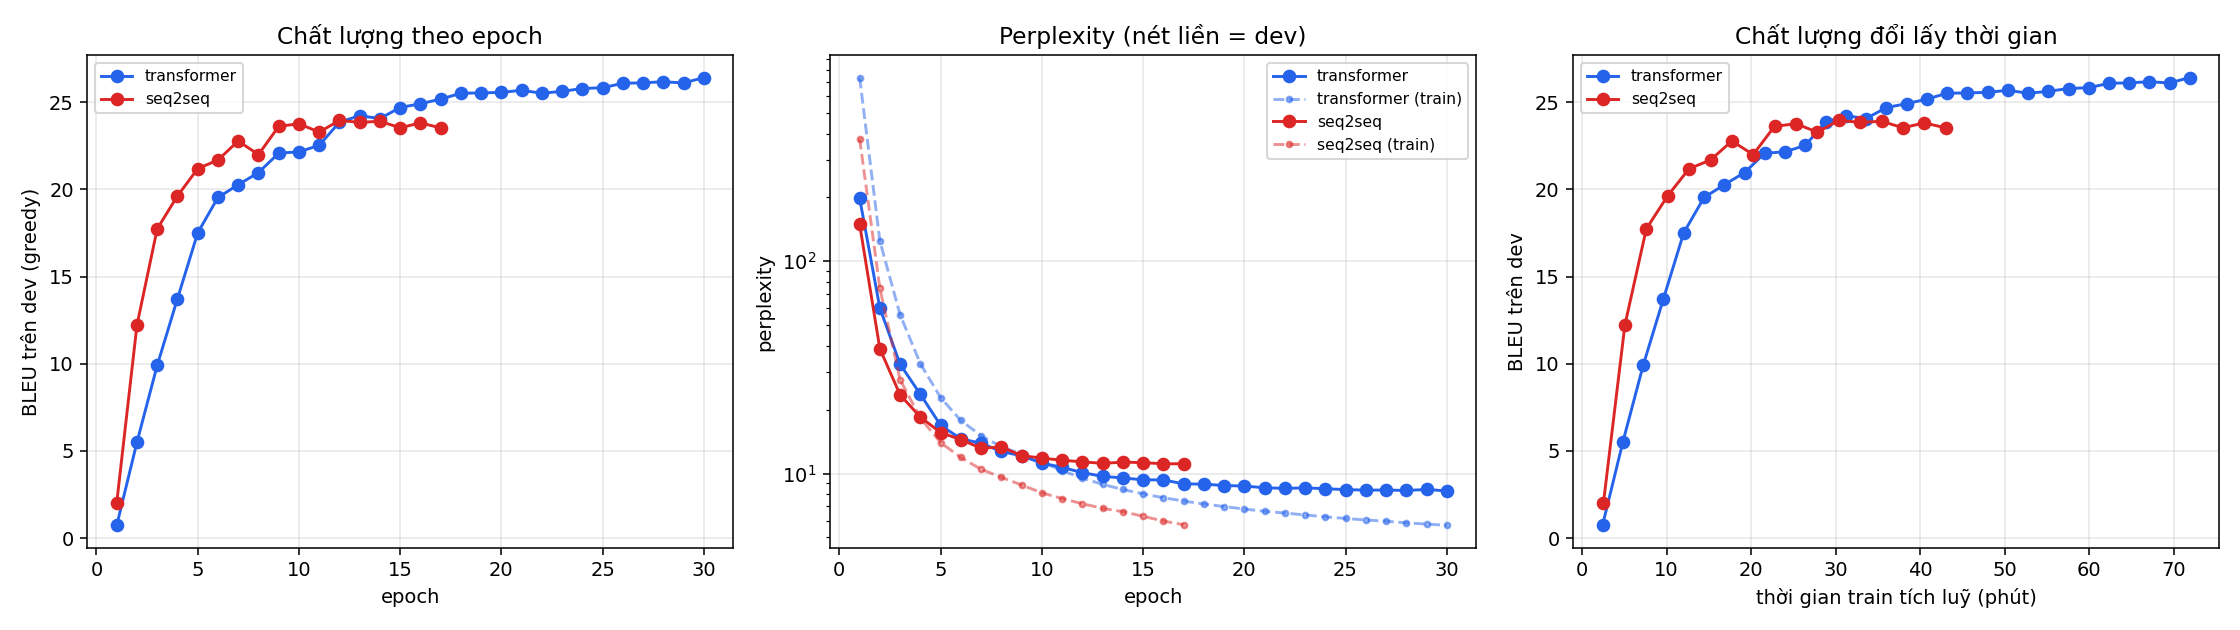
\includegraphics[width=\textwidth]{../results/comparison.png}
\caption{Từ trái sang phải: BLEU trên tập phát triển theo Epoch; Perplexity theo
Epoch (nét liền là Validation, nét đứt là Training); BLEU đổi lấy thời gian huấn
luyện tích luỹ.}
\label{fig:comparison}
\end{figure}

% =====================================================================
\section{Kết luận}
\label{sec:ketluan}

Báo cáo đã cài đặt lại hai kiến trúc NMT trên cùng ngữ liệu IWSLT'15
English--Vietnamese và so sánh chúng trong điều kiện kiểm soát. Cả hai bản cài
đặt đều vượt mốc tham chiếu tương ứng, xác nhận tính trung thành với kiến trúc
gốc.

\subsection{Các kiến trúc và kỹ thuật đã áp dụng}

Bảng~\ref{tab:applied} liệt kê chính xác thành phần nào trong mã nguồn được lấy
từ công trình nào.

\begin{table}[H]
\centering
\small
\caption{Ánh xạ giữa công trình tham khảo và mã nguồn}
\label{tab:applied}
\begin{tabularx}{\textwidth}{llXl}
\toprule
\textbf{Nguồn} & \textbf{Tên gọi} & \textbf{Thành phần áp dụng} & \textbf{Vị trí} \\
\midrule
\cite{vaswani2017} & Transformer &
Kiến trúc Encoder--Decoder, Positional Encoding Sin/Cos, Label Smoothing,
Inverse-Sqrt Schedule & \file{translate\_transformers/} \\
\addlinespace
\cite{sennrich2016} & BPE &
Phân đoạn Subword & \file{common/tokenizer.py} \\
\addlinespace
\cite{luong2015emnlp} & Global Attention &
Ba hàm điểm \file{dot}/\file{general}/\file{concat}, Input Feeding
& \file{translate\_seq2seq/} \\
\addlinespace
\cite{luong2015iwslt} & Stanford-NMT &
Quy ước chia tập train / tst2012 / tst2013 & \file{common/data.py} \\
\addlinespace
\cite{phanvu2017} & --- &
Bỏ bước tách từ tiếng Việt & \file{scripts/prepare.py} \\
\addlinespace
\cite{ott2018} & Scaling-NMT &
fp16, chia Batch theo Token, Gradient Accumulation
& \file{common/data.py}, \file{common/engine.py} \\
\addlinespace
\cite{nguyen2019} & TwT &
Pre-Norm Residual & \file{translate\_transformers/} \\
\addlinespace
\cite{wu2016} & GNMT &
Length Penalty cho Beam Search & cả hai tệp \file{model.py} \\
\addlinespace
\cite{tfnmt} & TF-NMT &
Toàn bộ siêu tham số của trường hợp 2 & \file{translate\_seq2seq/config.py} \\
\bottomrule
\end{tabularx}
\end{table}

Hai kỹ thuật ScaleNorm và FixNorm của TwT~\cite{nguyen2019} chưa được cài đặt.
Các phương pháp xử lý Rare Word trong~\cite{nguyen2019rare} cũng chưa được áp
dụng, do vấn đề này đã được giải quyết một phần bằng BPE.

\subsection{Kết luận chính}

Thứ nhất, Transformer cho chất lượng dịch cao hơn Seq2Seq--LSTM \textbf{2,54}
điểm BLEU trong cùng điều kiện (\textbf{30,35} so với \textbf{27,81}), và khoảng
cách thực tế còn lớn hơn vì Transformer chưa hội tụ khi dừng.

Thứ hai, lợi thế tốc độ huấn luyện thường được gán cho Transformer không xuất
hiện ở quy mô mô hình và phần cứng của thí nghiệm này. Số tham số và chi phí
Self-Attention bậc hai bù trừ cho lợi thế song song hoá.

Thứ ba, chất lượng của một hệ thống dịch máy phụ thuộc nhiều vào các lựa chọn
nằm ngoài kiến trúc. Việc chuyển từ từ điển mức từ sang BPE~\cite{sennrich2016},
và từ SGD sang Adam, đủ để đưa một kiến trúc từ năm 2015 vượt qua con số công bố
của chính nó thêm \textbf{1,71} điểm BLEU.

\subsection{Hướng phát triển}

Ba hướng có thể nâng kết quả. Thứ nhất, huấn luyện \ours{}-TF tới khi hội tụ
thật sự, ước tính đạt \textbf{31} đến \textbf{32} BLEU dựa trên xu hướng của
những Epoch cuối. Thứ hai, bổ sung ScaleNorm và FixNorm~\cite{nguyen2019}, vốn
là phần còn lại của công trình đã lập mốc \textbf{32,8} BLEU trên chính ngữ liệu
này. Thứ ba, thêm Key/Value Cache cho hàm Decoding của Transformer, nhằm loại bỏ
khoảng cách \textbf{37,7} lần về tốc độ suy luận vốn không phải bản chất của
kiến trúc.

% =====================================================================
\begin{thebibliography}{99}
\small

\bibitem{vaswani2017}
A. Vaswani, N. Shazeer, N. Parmar, J. Uszkoreit, L. Jones, A. N. Gomez,
Ł. Kaiser, and I. Polosukhin, ``Attention Is All You Need,'' in
\emph{Advances in Neural Information Processing Systems 30 (NeurIPS)}, 2017,
pp. 5998--6008. \url{https://arxiv.org/abs/1706.03762}

\bibitem{sennrich2016}
R. Sennrich, B. Haddow, and A. Birch, ``Neural Machine Translation of Rare Words
with Subword Units,'' in \emph{Proc. 54th Annual Meeting of the Association for
Computational Linguistics (ACL)}, Berlin, 2016, pp. 1715--1725.
\url{https://aclanthology.org/P16-1162/}

\bibitem{luong2015emnlp}
M.-T. Luong, H. Pham, and C. D. Manning, ``Effective Approaches to
Attention-based Neural Machine Translation,'' in \emph{Proc. Conference on
Empirical Methods in Natural Language Processing (EMNLP)}, Lisbon, 2015,
pp. 1412--1421. \url{https://aclanthology.org/D15-1166/}

\bibitem{luong2015iwslt}
M.-T. Luong and C. D. Manning, ``Stanford Neural Machine Translation Systems for
Spoken Language Domains,'' in \emph{Proc. 12th International Workshop on Spoken
Language Translation (IWSLT)}, Đà Nẵng, 2015, pp. 76--79.
\url{https://aclanthology.org/2015.iwslt-evaluation.11/}

\bibitem{phanvu2017}
H.-H. Phan-Vu, V. T. Tran, V. N. Nguyen, H. V. Dang, and P. T. Do, ``Towards
State-of-the-art English-Vietnamese Neural Machine Translation,'' in \emph{Proc.
8th International Symposium on Information and Communication Technology
(SoICT)}, 2017. \url{https://dl.acm.org/doi/10.1145/3155133.3155205}

\bibitem{phanvu2019}
H.-H. Phan-Vu, V. T. Tran, V. N. Nguyen, H. V. Dang, and P. T. Do, ``Neural
Machine Translation between Vietnamese and English: an Empirical Study,''
\emph{Journal of Computer Science and Cybernetics}, vol. 35, no. 2,
pp. 147--166, 2019. \url{https://vjs.ac.vn/index.php/jcc/article/view/13233}

\bibitem{ott2018}
M. Ott, S. Edunov, D. Grangier, and M. Auli, ``Scaling Neural Machine
Translation,'' in \emph{Proc. Third Conference on Machine Translation (WMT)},
Brussels, 2018, pp. 1--9. \url{https://aclanthology.org/W18-6301/}

\bibitem{nguyen2019}
T. Q. Nguyen and J. Salazar, ``Transformers without Tears: Improving the
Normalization of Self-Attention,'' in \emph{Proc. 16th International Conference
on Spoken Language Translation (IWSLT)}, Hong Kong, 2019.
\url{https://aclanthology.org/2019.iwslt-1.17/}

\bibitem{wu2016}
Y. Wu, M. Schuster, Z. Chen, Q. V. Le, M. Norouzi \emph{et al.}, ``Google's
Neural Machine Translation System: Bridging the Gap between Human and Machine
Translation,'' arXiv:1609.08144, 2016. \url{https://arxiv.org/abs/1609.08144}

\bibitem{bahdanau2015}
D. Bahdanau, K. Cho, and Y. Bengio, ``Neural Machine Translation by Jointly
Learning to Align and Translate,'' in \emph{Proc. International Conference on
Learning Representations (ICLR)}, San Diego, 2015.
\url{https://arxiv.org/abs/1409.0473}

\bibitem{tran2015}
V. H. Tran, H. T. Vu, T. T. Le, L. N. Pham, and V. V. Nguyen, ``The
English-Vietnamese Machine Translation System for IWSLT 2015,'' in \emph{Proc.
12th International Workshop on Spoken Language Translation: Evaluation Campaign
(IWSLT)}, Đà Nẵng, 2015, pp. 80--83.
\url{https://aclanthology.org/2015.iwslt-evaluation.12/}

\bibitem{nguyen2019rare}
T.-V. Nguyen, L.-M. Nguyen, P.-T. Nguyen \emph{et al.}, ``Overcoming the Rare
Word Problem for Low-Resource Language Pairs in Neural Machine Translation,'' in
\emph{Proc. 6th Workshop on Asian Translation (WAT@ACL)}, Hong Kong, 2019,
pp. 207--214. \url{https://aclanthology.org/D19-5228/}

\bibitem{tfnmt}
TensorFlow, ``Neural Machine Translation (seq2seq) Tutorial,''
\url{https://github.com/tensorflow/nmt}

\bibitem{sutskever2014}
I. Sutskever, O. Vinyals, and Q. V. Le, ``Sequence to Sequence Learning with
Neural Networks,'' in \emph{Advances in Neural Information Processing Systems 27
(NeurIPS)}, 2014, pp. 3104--3112. \url{https://arxiv.org/abs/1409.3215}

\bibitem{zhang2019}
M. Zhang, Z. Li, G. Fu, and M. Zhang, ``Syntax-Enhanced Neural Machine
Translation with Syntax-Aware Word Representations,'' in \emph{Proc. 2019
Conference of the North American Chapter of the Association for Computational
Linguistics: Human Language Technologies (NAACL-HLT)}, Minneapolis, 2019,
pp. 1151--1161. \url{https://aclanthology.org/N19-1118/}

\end{thebibliography}

% =====================================================================
\appendix
\section{Tái hiện kết quả}

Mã nguồn: \url{https://github.com/quanai06/machine_translate}

\begin{verbatim}
git clone https://github.com/quanai06/machine_translate.git
cd machine_translate
pip install -r requirements.txt
bash scripts/download_data.sh      # tải và kiểm tra ngữ liệu
python scripts/prepare.py          # train Tokenizer dùng chung
python scripts/check_amp.py        # kiểm tra Mixed Precision
python scripts/sanity_check.py     # kiểm tra Overfitting có chủ đích
python translate_transformers/train.py
python translate_seq2seq/train.py
python compare.py --plots
\end{verbatim}

Trên Google Colab, mở \file{notebooks/colab\_full.ipynb} và chọn GPU T4.

Toàn bộ nhật ký của lần chạy tạo ra các số liệu trong báo cáo được lưu trong
\file{notebooks/translate\_colab\_run.ipynb}. Bảng so sánh và biểu đồ do
\file{compare.py} sinh ra nằm trong thư mục \file{results/}.

\end{document}
